% !TeX spellcheck = en_US
\documentclass{bioinfo}

\usepackage{hyperref} \usepackage{tikz} \usetikzlibrary{graphs}

\let\proglang=\textsf

\copyrightyear{2016} \pubyear{2016}

\begin{document} \firstpage{1}
	
\title[RDML]{RDML: an \textbf{R} Package for Working with RDML Format Data}
\author[Blagodatskikh \textit{et~al}]{Konstantin Blagodatskikh\,$^{1}$\footnote{to whom correspondence should be addressed}, Micha\l{} Burdukiewicz\,$^{2}$, Stefan R\"{o}diger\,$^{3}$ 
	and Andrej-Nikolai Spiess\,$^{4}$} 

\address{$^{1}$Evrogen JSC, Moscow, Russia\\ 
	 $^{2}$Department of Genomics, Faculty of Biotechnology, University of Wroc\l{}aw, Wroc\l{}aw, Poland\\
	 $^{3}$Institute of Biotechnology, Brandenburg University of Technology Cottbus--Senftenberg, Senftenberg, Germany\\ 
	 $^{4}$University Medical Center Hamburg-Eppendorf, Hamburg, Germany
	 }
	
\history{Received on XXXXX; revised on XXXXX; accepted on XXXXX}

\editor{Associate Editor: XXXXXXX}
	
\maketitle

\begin{abstract}
		
\section{Motivation:} Reproducible research is essential in science. 
Part of this is are open standards for data exchange, which preserve 
the set-up and output of experiments in defined schemes. The Real-time PCR 
Data Markup Language (RDML) is a recommended standard of the Minimum Information 
for Publication of Quantitative Real-Time PCR Experiments (MIQE) guidelines. 
Despite the fact that software products of qPCR instruments export RDML data, 
there is no tool designed for working with RDML data in sophisticated 
environment for statistical bioinformatics.
		
\section{Results:} We developed the cross-platform open source \textit{RDML} 
package for the statistical computing language \textbf{R}. \textit{RDML} is 
compliment to RDML~$\geq$~v.~1.2 and provides functionality to (i) import RDML 
data; (ii) to extracts sample information (e.g., targets, concentration); (iii) 
to transform data to various formats of the \textbf{R} environment; (iv) to 
generate human readable experiment summaries; and (v) to create RDML files from 
user data. In addition, offers \textit{RDML} a graphical user interface to read, 
edit and create RDML files. We show that \textit{RDML} enables a seamless analysis with 
with other \textbf{R} packages.

\section{Availability:} url{https://cran.r-project.org/package=RDML}. Source code: 
url{https://github.com/kablag/RDML}. \section{Contact:} 
\href{k.blag@yandex.ru}{k.blag@yandex.ru} \end{abstract}


\section{Introduction}
  Real-time quantitative PCR (qPCR) is one of the most used methods in molecular 
biology, diagnostics and other areas. qPCR is well accepted since 
it is simple, accurate, reliable and reproducible \cite{pabinger_2014}. The 
Minimum Information for Publication of Quantitative Real-Time PCR Experiments
were established to facilitate the comparison of experimental results from qPCRs 
\cite{huggett_2013}. There are at least twenty qPCR cycler manufacturers. Such variety creates a broad selection to 
address the specific market demands. The systems differ in details such as the 
number of processable samples, the number of detection channels, the sample 
arrangement (e.g., plate, carousel). Moreover, the devices use different 
data processing methods and non-interchangeable storage formats (e.g.,  binary formats). 
Binary data formats and system specific formats result in most cases a vendor 
lock-in. Therefore, the diversification comes at a cost at the level of data 
exchange. Discrepancies in data processing hinder comparison of the PCR results 
obtained on different systems. Disparate storage formats prohibit the processing 
of raw data from one instrument in the another system. Data processing is a 
central challenge in qPCR data analysis \cite{bustin_reproducibility_2014, roediger2015r, 
spiess_impact_2014, spiess_system-specific_2016}.

The MIQE guidelines suggest the Real-time PCR Data Markup Language (RDML) as 
qPCR interchange data format \cite{rdml-ninja_2015}. RDML is a vendor 
independent and freely available file format. The RDML format is based on 
eXtensible Markup Language (XML), which is commonly used in bioinformatics 
\cite{achard_xml_2001}, to pass meta data and values between applications. 
Storage and exchange of qPCR data is bidirectional. The RDML data standard 
contains the primary raw data acquired by the machine, meta-information to 
understand the experimental setup (e.g., sample annotation, qPCR protocol, probe 
and primer sequences) and information to re-analyse the data 
\cite{lefever_rdml_2009}. The RDML format is supported by different vendors (see 
Supplement) and third-party software (e.g., \textit{Primer3Plus} 
\cite{untergasser_2007}, \textit{QPCR}, \textit{LinRegPCR}, \textit{qBase+}) 
\cite{pabinger_2014, rdml-ninja_2015}. Despite the openness of the RDML format, 
there was is no open source software capable of reading, processing and writing 
this format. Users have to choose between programs from manufacturers of PCR 
devices (which can use only their own generated files) or commercial software 
such as \textit{qbase+} \cite{pabinger_2014, rdml-ninja_2015}. Recently, 
Ruijter~\textit{et~al.} published the open-source desktop software 
\textit{RDML-Ninja}, which can visualize, edit and validate RDML files 
\cite{rdml-ninja_2015}. However, \textit{RDML-Ninja} cannot analyze the qPCR 
data by sophisticated analysis pipelines. This limits its applications in 
customized high-throughput applications. Moreover, there is a need for a \textit{de novo} 
creation of RDML data.  It is especially of importance for systems, that do not 
support the RDML format (e.g., commercial systems, prototypes, point-of-care devices). 

The cross-platform statistical computing language \textbf{R} is a \textit{de facto} standard in applied 
statistical bioinformatics provides comprehensive tool-sets for reproducible \cite{leeper_archiving_2014, 
liu_r_2014, roediger2015r} and is suitable for standalone desktops or servers \cite{roediger2015r}. 
There is a number of \textbf{R} packages for qPCR and melting 
curve analysis written in \cite{pabinger_2014, ritz_qpcr_2008, 
roediger_RJ_2013, roediger2015chippcr}. Although the \textbf{R} environment 
extended by dedicated packages provides wide array of tools, it was not possible 
to seamlessly process RDML files.

The common approaches for data management in \textbf{R} are native formats such 
as and \textbf{R} workspaces or objects \cite{roediger_rkward_2012}. However, 
the external applications of these methods is limited regarding the RDML format, 
a specifically tailored variant of XML. The principle of reproducible research 
is not retained without a standard method of data import as the \textit{RDML} 
package. Our software enables usage of the qPCR-related \textbf{R} tools as 
recently reviewed in \cite{pabinger_2014}, while working on the RDML data 
derived straight from the PCR system. Concluding, the \textit{RDML} package may 
serve as foundation for other \textbf{R} package hosted at Bioconductor 
\cite{gentleman_2004} and CRAN as it was shown recently in \cite{roediger2015r}.

Here, we describe the \textit{RDML} package, which 
allows to exchange RDML files ($\geq$~v.~1.1) and transform it to the human 
readable format. Until version \textit{RDML} package 0.8-3, only RDML~v.~1.1 and 
file import was supported. Here we present a considerably maturated version of 
the package including a novel GUI to read, edit and create RDML files. \textit{RDML} package is open-source, free to use, 
platform-independent, and thus can be modified for specific tasks or other 
\textbf{R} packages, or even integrated to work-flows with other programming 
languages. Despite many qPCR instruments and software solutions are able 
to work with the RDML format, there is a need make RDML available for the increasingly 
used \textbf{R} environment.

\section{Implementation}
	
The \textit{RDML} package is available at CRAN 
(\url{https://cran.r-project.org/package=RDML}) and the 
development version is hosted at GitHub (\url{https://github.com/kablag/RDML}) 
with facilities for bugs reports and request features. \textit{RDML} provides 
\emph{R6} classes, which corresponds to RDML~v.~1.2 input format types. 


chaining function \emph{R6}

\textbf{R} 
is a language with dynamic typing. This is helpful while scripting but can lead 
to problematic debugging of more complicated workflows. \emph{R6} classes 
provide type-safe interfaces to set data without access to inner structure of 
objects thus all imputed data can be validated. This option is very useful when 
creating packages to work as intermediate level for other packages (e.g., such 
approach does not allow set \emph{character} in place of \emph{integer} 
Supplementary Section S3.3). Furthermore, the inheritance of \emph{R6} objects 
unifies the structure of the package and streamlines extending its capabilities 
(the whole package is written around a single base class). The main interaction 
is via the command line interface (CLI). This enables batch processing. However, we designed the graphical user
interface \textbf{rdmlEdit} based on the \textit{shiny} technology as described in \cite{roediger2015chippcr}. This GUI allows to edit RDML meta data and view fluorescence
curve (Fig.~\ref{fig:02}). The RDML file format, coordinated by the RDML consortium (www.rdml.org/), is under continuous development. The \textit{RDML} 
package follows the changes and supports the current version RDML~v.~1.2. 
Central functionality of the \textit{RDML} package encompass the read-in of RDML 
data file and summary generation for RDML objects. The capabilities of packages 
range from advanced statistical analysis to simple yet crucial extraction of the 
fluorescence data. The public methods of the main class called RDML can be used 
to access and process the RDML data. These methods include:

\begin{itemize} 
  \item \textbf{\$new()} -- creates new RDML object. Empty or from specified RDML 
  file (Supplementary Section S3.1 and S3.10-3.13);
  \item \textbf{\$AsDendrogram()} -- represents 
  structure of RDML object as dendrogram (Fig.~\ref{fig:01}) to observe it. (\ref{fig:01} and Supplementary Section 
  S3.1);
  \item \textbf{\$AsTable()} -- represents data contained in RDML object (except 
  fluorescent data) as \textit{data.frame} (Supplementary Section S3.4);
  \item \textbf{\$GetFData()} -- gets fluorescent data (Supplementary Section S3.5);
  \item \textbf{\$SetFData()} -- sets fluorescent data to RDML object (Supplementary Section S3.6); 
  \item \textbf{\$AsXML()} -- saves RDML object as RDML~v.~1.2 file (Supplementary Section S3.8).
\end{itemize}
	
	Beside working with existing RDML files, the package can create new RDML 
objects from the data obtained from systems that do not support RDML format. To 
create eligible RDML object, one has to provide fluorescence data and minimal 
description of experiment (Supplementary Section S3.10). The another unique feature of our 
package is the ability to merge several RDML files (experiments) into one with 
\textbf{MergeRDMLs()} function and process them like unit (\ref{fig:01} and Supplementary Section 
S3.7). For example, you can combine results of two runs that have sample from one 
experiment or add calibration samples from one run to another.

Data sets are an essential element of \textbf{R} packages for reproducible 
research \cite{roediger2015r}. As of \textit{RDML} v.~0.9-5 we provide data sets 
from the Bio-Rad CFX 96, Roche LightCycler 96 and Applied Biosystems StepOne.

\begin{figure}
	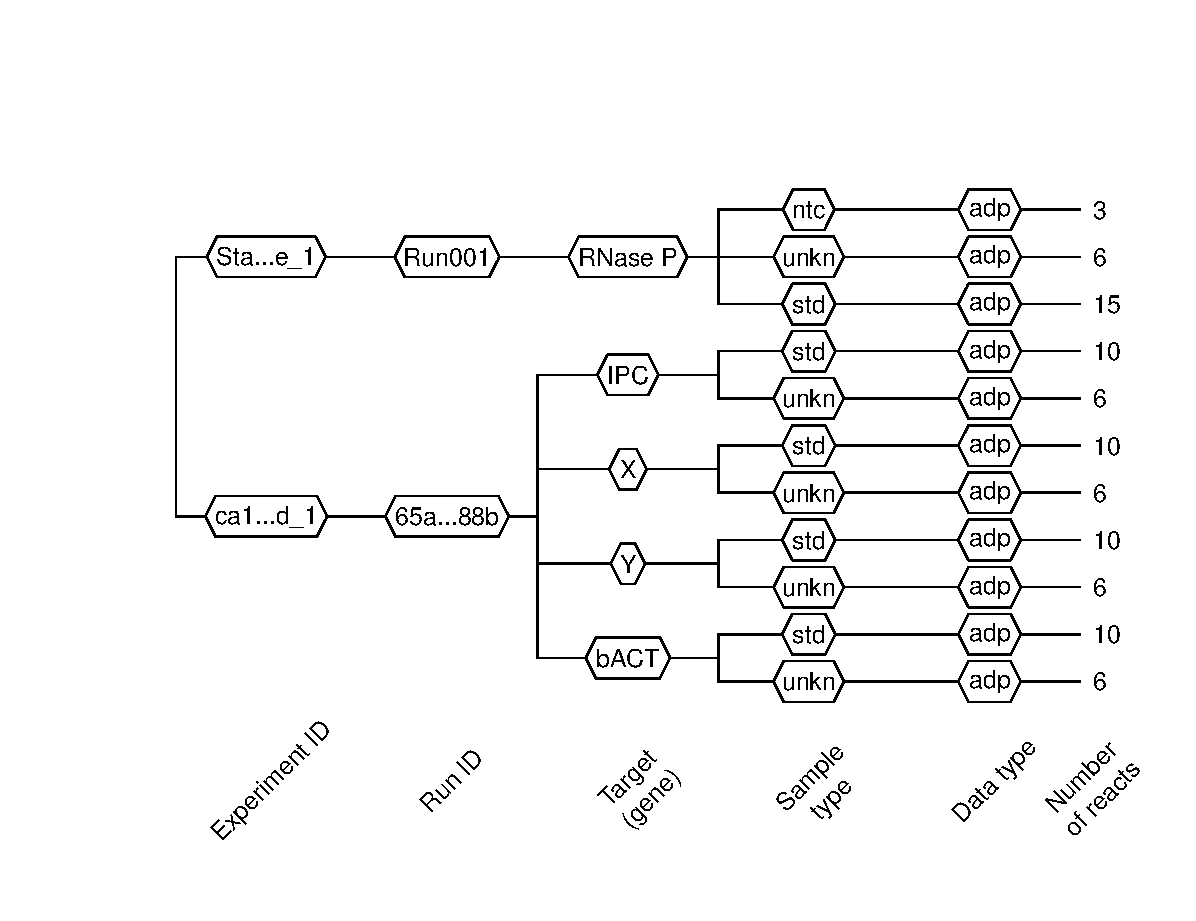
\includegraphics[width=0.5\textwidth]{as_dendrogram.eps}
	\caption{Structure of RDML object represented as dendrogram via the 
	  \textbf{\$AsDendrogram()} function. Two files 
	  were loaded and merged into one object. As a result two 
	  experiments can be processed in one pipeline.}\label{fig:01}
\end{figure}
\begin{figure}
	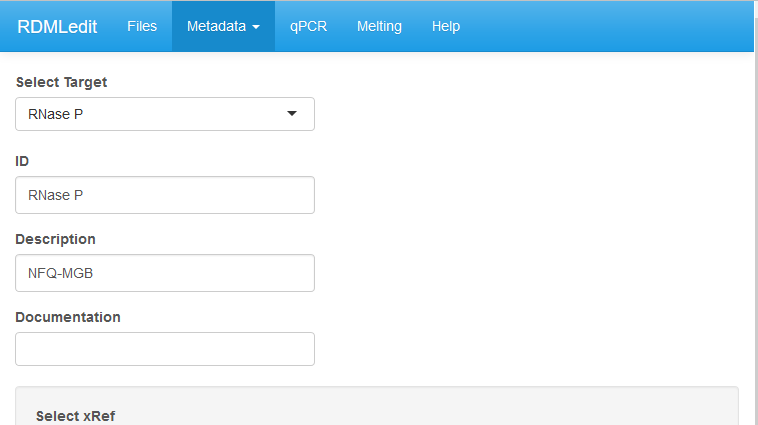
\includegraphics[width=0.5\textwidth]{target.PNG}
	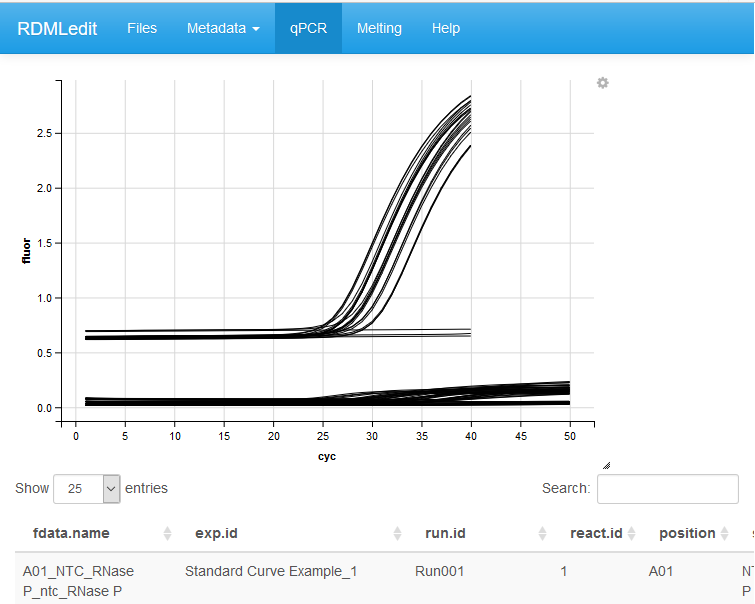
\includegraphics[width=0.5\textwidth]{adp.PNG}
	\caption{Working with RDML files in the \textbf{rdmlEdit} GUI. 
	  The function \textbf{rdmlEdit()} invokes a shiny GUI which allows for 
	  example to merge data, edit meta-data (e.g. (A) - Target), view raw 
	  data of the amplification and melting curves (B). Both the plot and 
	  the table are interactive with highlighting and filter features.}\label{fig:02}
\end{figure}


\section{Discussions and conclusions}
	
	The \textit{RDML} package for \textbf{R} imports and manipulates data 
from RDML~v.~1.1 and v.~1.2 format files. It can also create RDML~v.~1.2 files 
from data provided by an user. This package can be used as a part of the qPCR 
processing workflows or for preliminary summaries of experiments. Due to the 
openness of the format, we anticipate that other scientific disciplines might 
benefit from this implementation.

Researchers can no longer collect data in a single laboratory and are often are 
coerced to work with many data sets. Adaptable data management - aka. adaptive 
informatics - is relevant in cases where data from omics approaches and 
different assays (e.g., flow cytometry, digital PCR, NGS) need to be merged 
\cite{baker_quantitative_2012}. Due to the fact that RDML is based on XML it is 
possible to converge the file with other formats such as HDF 
\cite{millard_adaptive_2011} which is supported by \textbf{R} \cite{Fischer_HDF5}. This enables extended data storage 
and analysis, but also a higher level of the experimental data management.

\section{Acknowledgements}
Grateful thanks belong to the \textbf{R} community and the RDML consortium.
	
\paragraph{Conflict of Interest\textcolon} none declared.

%\bibliographystyle{natbib}
%\bibliographystyle{achemnat}
%\bibliographystyle{plainnat}
%\bibliographystyle{abbrv}
%\bibliographystyle{bioinformatics}
%
\bibliographystyle{plain}
%
\bibliography{RDML}

\end{document}
